%!TEX program = xelatex
\documentclass[titlepage,11pt,a4paper]{article}
\usepackage{amssymb}
\usepackage{dsfont}
\usepackage{graphicx}
\usepackage{amsmath}
\usepackage{subfig}
\usepackage[ruled,vlined]{algorithm2e}
\graphicspath{ {images/} }
\usepackage[titlepage]{polytechnique}


\title[MAP 411 MINI Project]{Effets du courant sur la dispersion d'un polluant}
    %\subtitle{Le sous-titre (optionnel, enlever cette ligne sinon)}
    \author{Jianfei \textsc{ZHANG}\\
            Zuli \textsc{HUANG}
            }
    \date{10/01/2017}


\begin{document}
%\maketitle

\section{Évolution de la concentration de pollant dans l'océan}
\subsection{Discrétisation du Laplacien en dimension 2}
On cherche à simuler via différences finies une fonction $u(x, y$ solution de l'équation de Laplace
\begin{equation}
\left\{
\begin{array}{lll}
-\Delta u(x,y) = f(x,y) & \forall (x, y) \in \Omega = ]0, L[ \times ]0, L[,\\
u(x, y) = 0 & \forall (x,y) \in \partial\Omega\\
\end{array}
\right.
\label{equ:equation_de_laplace}
\end{equation}

Pour résoudre numériquement cette équation, nous utilisons alors

-- $h$ le pas de discrétisation en espace commun aux deux directions;

-- $N=\frac L h -1$ la taille de la maille;

-- $x_i = ih$ et $y_j = jh$ les coordonnées des points de la maille, $0\leqslant i, j \leqslant N+1$;

-- $u_{i,j}$ l'approximation de $u(x_i, y_j)$;

-- $f_{i,j} = f(x_i, y_j)$ la discrétisation de $f$ aux points de la maille

On utilise pour calculer les $(u_{i,j})_{1\leqslant i,j\leqslant N}$ le schéma aux différence finies

$$
-\frac{u_{i-1, j} - 2u_{i,j} + u_{i+1, j}}{h^2} - \frac{u_{i, j-1} - 2u_{i,j} + u_{i, j+1}}{h^2} = f_{i,j}, \mbox{ avec }1\leqslant i,j\leqslant N.
$$

On introduit le vecteur U de taille $N^2$ qui est donné par la concaténation des lignes de la matrice $(u_{i, j})_{1\leqslant i, j \leqslant N}$:

$$
U_{(i-1)N + j}=u_{i,j} \mbox{ pour } 1 \leqslant i, j\leqslant N.
$$

\subsubsection{Q9}
Calculer la matrice $A$ et le vecteur $b$ pour lesquels $U$ est solution du système linéaire

\begin{equation}
-AU = b.
\label{equ:equation_numerique_laplace}
\end{equation}

D'après le schéma qu'on introduit à l'énoncé, on obtient que

$$
-\frac 1 {h^2} (u_{i-1,j} + u_{i+1,j} - 4u_{i,j} + u_{i,j-1} + u_{i,j+1}) = f_{i,j}.
$$

Alors, on peut facilement en déduire la forme explicite de $b$ et celle de $A$.
Pour décrire la matrice $A$, d'abord, on note deux matrices : $M$ et $I$.

$$
  M =
  \begin{pmatrix}
   -\frac 4 {h^2} &  \frac 1 {h^2}&  &0\\
   \frac 1 {h^2}& \ddots & \ddots &\\
   &  \ddots& \ddots &\frac 1 {h^2}\\
   0&  &   \frac 1 {h^2}&   -\frac 4 {h^2}\\
  \end{pmatrix}_{N\times N}
$$

$$
  I =
  \begin{pmatrix}
   \frac 1 {h^2} &  &  &0\\
   & \ddots &  &\\
   &  & \ddots &\\
   0&  &   &   \frac 1 {h^2}\\
  \end{pmatrix}_{N\times N}
$$

Alors, on peut donner l'expression de $A$ en utilisant $M$ et $I_d$.

$$
  A =
  \begin{pmatrix}
   M &  I&  &0\\
   I& \ddots & \ddots &\\
   &  \ddots& \ddots &I\\
   0&  &   I&   M\\
  \end{pmatrix}_{N^2\times N^2}
$$

Dans ce cas là, on obtient le vecteur $b$ de la taille $N^2$.

$$
b_{(i-1)N + j} = f_{i,j} \mbox{ pour } 1 \leqslant i, j\leqslant N.
$$

Grace à $A$ et $b$, on peut résoudre numériquement l'equantion de Laplace avec un terme source bien choisi permettant de comparer la résolution numérique et la solution exacte. Ici, on prend le terme source la forme polynomiale.

$$
f(x, y) = -2x(x-L)-2y(y-L)
$$

Par conséquent, on a la solution exacte :

$$
u(x, y) = x(x-L)y(y-L)
$$

Puis, on choisit $h = 0.01$ et $L = $. Or, on peut résoudre numériquement l'equation de Laplace et obtenir le Figure \ref{fig:numerical_result}.

\begin{figure}[h]
\centering
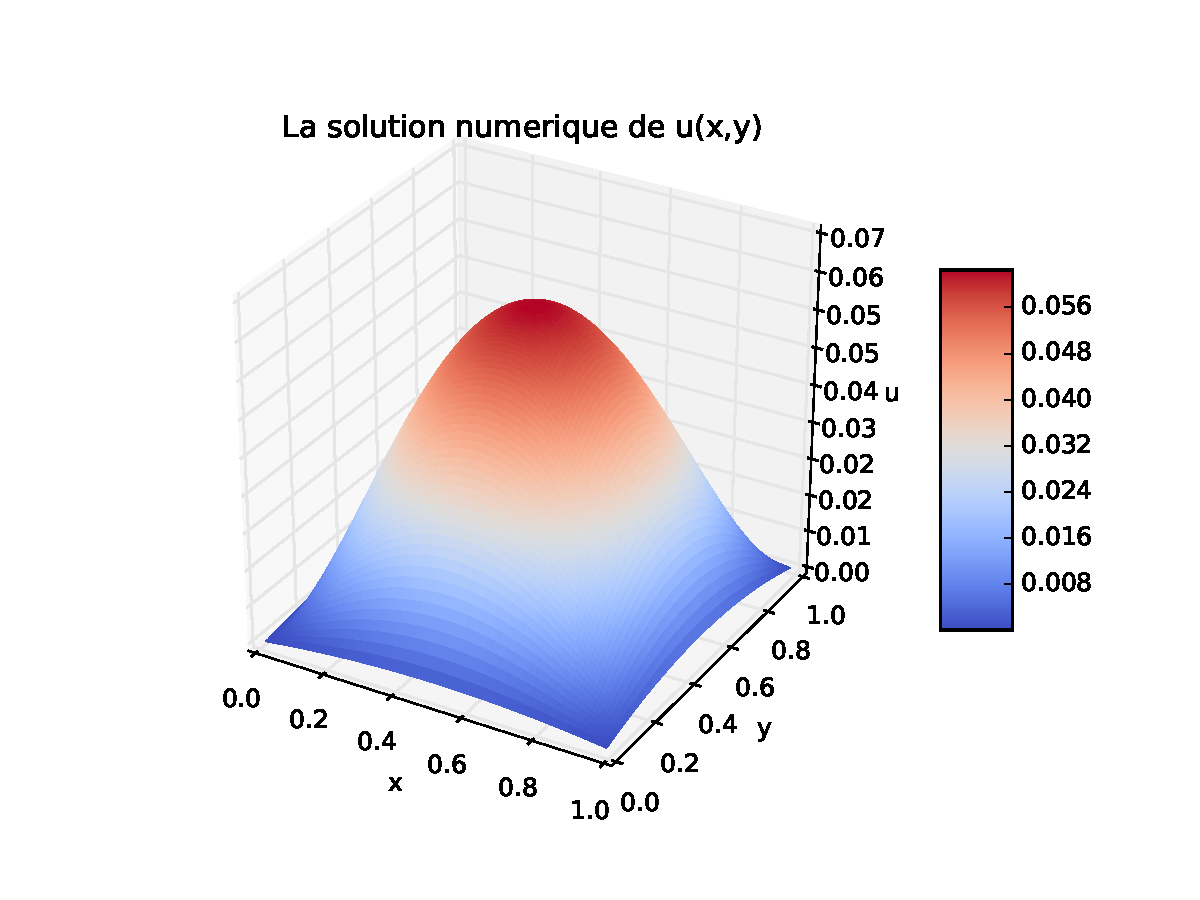
\includegraphics[width=0.85\textwidth]{Q_9.pdf}
\caption{Résultat numérique de l'equation \ref{equ:equation_numerique_laplace}}
\label{fig:numerical_result}
\end{figure}
\newpage


Nous montrons également le dessin de la solution théorique ci-dessous. Nous pouvons voir que la solution, qu'on a obtenu par la méthode numérique, approche bien la solution exacte.

\begin{figure}[h]
\centering
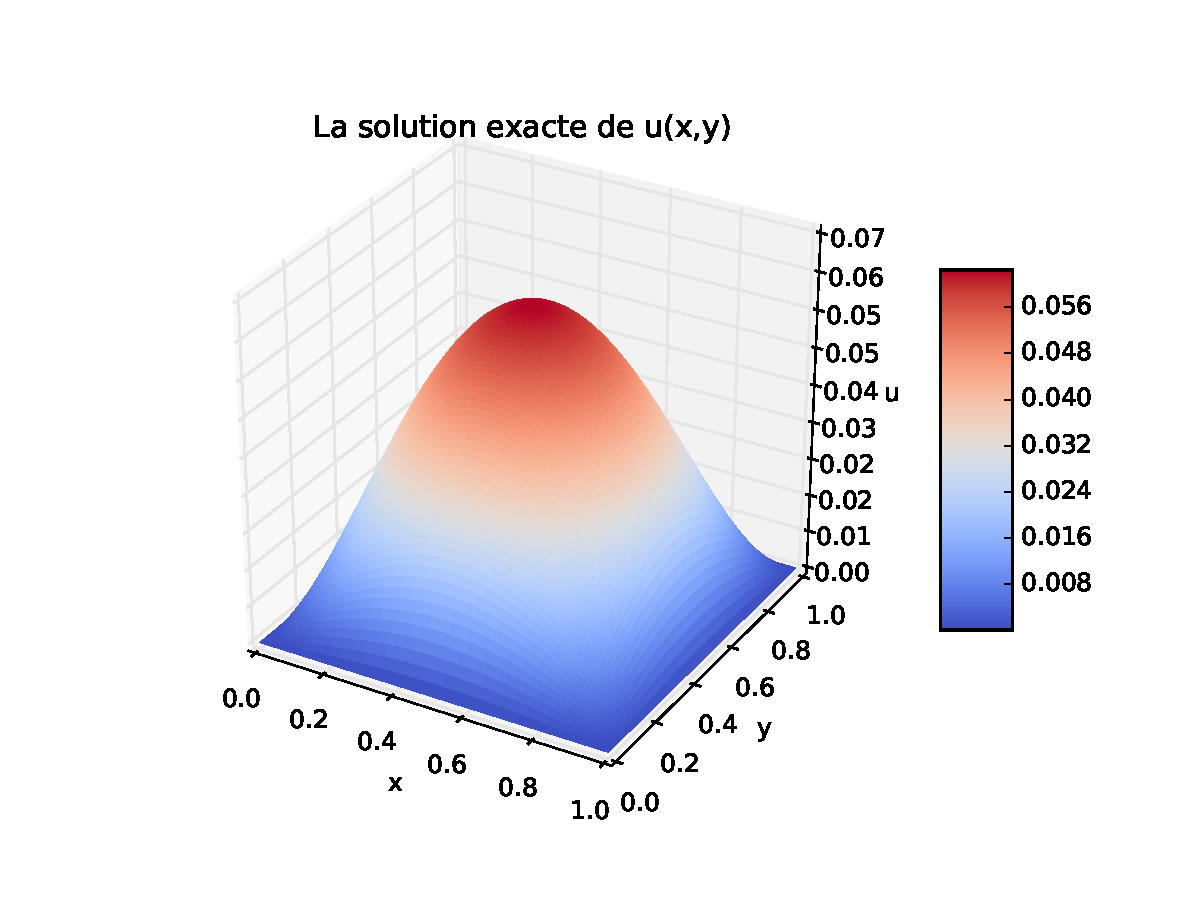
\includegraphics[width=0.85\textwidth]{Q_9_exacte.pdf}
\caption{Résultat théorique de l'equation \ref{equ:equation_numerique_laplace}}
\label{fig:theoretical_result}
\end{figure}

Pour obtenir l'ordre de convergence du schméma, on peut calculer l'erreur de troncature. Evidemment, ce schéma est de l'ordre 2 en espace.

$$
\begin{array}{lll}

\eta_{i,j} &=& -\displaystyle\frac{u_{i-1, j} - 2u_{i,j} + u_{i+1, j}}{h^2} - \displaystyle\frac{u_{i, j-1} - 2{i,j} + u_{i, j+1}}{h^2} +\\

&&\displaystyle\frac{u(x_{i-1}, y_j) - 2u(x_i,y_j) + u(x_{i+1}, y_j)}{h^2} + \displaystyle\frac{u_(x_i, y_{j-1}) - 2u(x_i,y_j) + u(x_i, y_{j+1})}{h^2}\\
&=&O(h^2)

\end{array}
$$

En choisissant différent $h$, l'on peut calculer l'écart entre la solution exacte et celle de théorique sous la norme 2.

$$
\mbox{erreur} = \sqrt{\sum_{i=1}^{N}\sum_{j=1}^{n}(u_{i,j} - u(x_i, y_j))^2 \times h^2}
$$

D'où, on obtient le figure de convergence.

\begin{figure}[h]
\centering
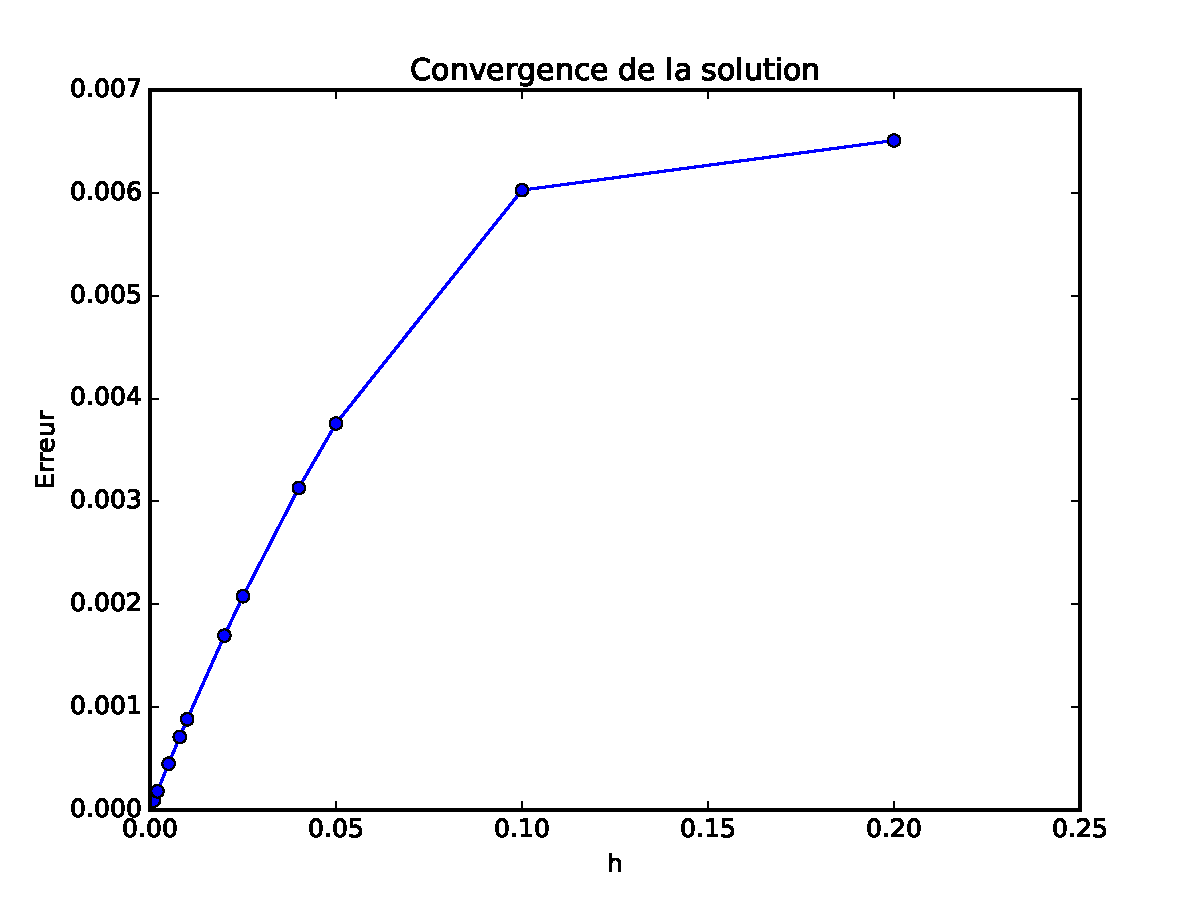
\includegraphics[width=0.85\textwidth]{Q_9_evolution.pdf}
\caption{Convergence du schéma}
\label{fig:convergence_scheme}
\end{figure}


\subsection{Équation de convection diffusion bi-dimensionnelle}
Nous pouvons à présent simuler le comportement de la concentration de polluant lorsqu'il est déversé dans l'océan par le fleuve. On modélise son évolution par l'équation de réaction diffusion sur un domaine $\Omega =]0, L[\times]0, L[$ avec conditions de Dirichlet au bord :

\begin{equation}
\left\{
\begin{array}{lll}
\displaystyle\frac{\partial u}{\partial t} + V^x \displaystyle\frac{\partial u}{\partial x} + V^y \displaystyle\frac{\partial u}{\partial y}-\nu\displaystyle\frac{\partial^2 u}{\partial x^2} -\nu\displaystyle\frac{\partial^2 u}{\partial y^2}= 0 & \forall (x, y) \in \Omega, \forall t > 0,\\
u(t=0, x, y) = u_0(x,y), & \forall (x,y) \in \Omega\\
u(t, x, y) = 0, & \forall (x,y) \in \partial\Omega\\
\end{array}
\right.
\label{equ:equation_de_laplace_temps}
\end{equation}

Pour résoudre numériquement cette équation nous utilisons de plus

-- $\Delta t$ le pas de discrétisation en temps ;

-- $t^n = n\Delta t$ les coordonnées du maillage temporel ;

-- $u^n_{i,j}$ l'approximation de $u(t^n, x_i, y_j)$ ;

-- $V^x_{i,j} = V^x(x_i,y_j)$ et $V^y_{i,j} = V^y(x_i,y_j)$ l'approximation de $u(t^n, x_i, y_j)$ la discrétisation de $V = (V^x, V^y)$ ;

-- $U^n$ de taille $N^2$ donné par la concaténation des lignes de la matrice $(u^n_{i,j})_{1\leq i, j \leq N}$, pour chaque $n\in \mathbb{N}$

\subsubsection{Q10}
D'après le schéma de Crank-Nicholson correspondant qu'on a dans l'énoncé, on peut calculer les matrices $K^x_c$ et $K^y_c$ quand $V = (1,1)$ pour l'équation ci-dessous.

\begin{equation}
(I_N + \frac{\Delta t}{2}(K_c^x + K^y_c) - \frac{\nu \Delta t}{2}A)U^{n+1} = (I_N - \frac{\Delta t}{2}(K_c^x + K^y_c) + \frac{\nu \Delta t}{2}A)U^{n}
\label{equ:relation_recurrence}
\end{equation}

On note la matrice $E$
$$
  E_1 =
  \begin{pmatrix}
   \frac 1 {2h} & &  & 0\\
   & \ddots &&\\
   &  & \ddots &\\
   0&  &  &   \frac 1 {2h}\\
  \end{pmatrix}_{N\times N}
  \mbox{ et }
  E_2 =
  \begin{pmatrix}
   0 &\frac 1 {2h} &  & 0\\
   -\frac 1 {2h}& \ddots &&\\
   &  &   \ddots&\frac 1 {2h}\\
   0&  &  -\frac 1 {2h}&   0\\
  \end{pmatrix}_{N\times N}
$$

D'où, on obtient que

$$
  K^x_c =
  \begin{pmatrix}
   E_2 & &  & 0\\
   & \ddots &&\\
   &  & \ddots &\\
   0&  &  &   E_2\\
  \end{pmatrix}_{N^2\times N^2}
\mbox{ et }
  K^x_c =
  \begin{pmatrix}
   0 & E_1&  & 0\\
   E_1& \ddots&\ddots&\\
   &  \ddots& \ddots &E_1\\
   0&  &  E_1&   0\\
  \end{pmatrix}_{N^2\times N^2}
$$

\subsubsection{Q11}
On peut faire la simulation numérique en appliquant $\nu = 1, L = 50, T=5, h = 0.5, \Delta t = 0.2$ et la condition initiale $u_0 = f_{x_0, y_0, \sigma}$ pour
$$
f_{x_0, y_0, \sigma} = \frac{1}{\sigma\sqrt{2\pi}}exp(-\frac{(x-x_0)^2+(y-y_0)^2}{2\sigma^2})
$$
avec $x=x_0=25$ et $\sigma = 1$.

On peut finalement obtenir le figure de simulation.
\newpage
\begin{figure}
\centering
\subfloat[$t = 0$]{
  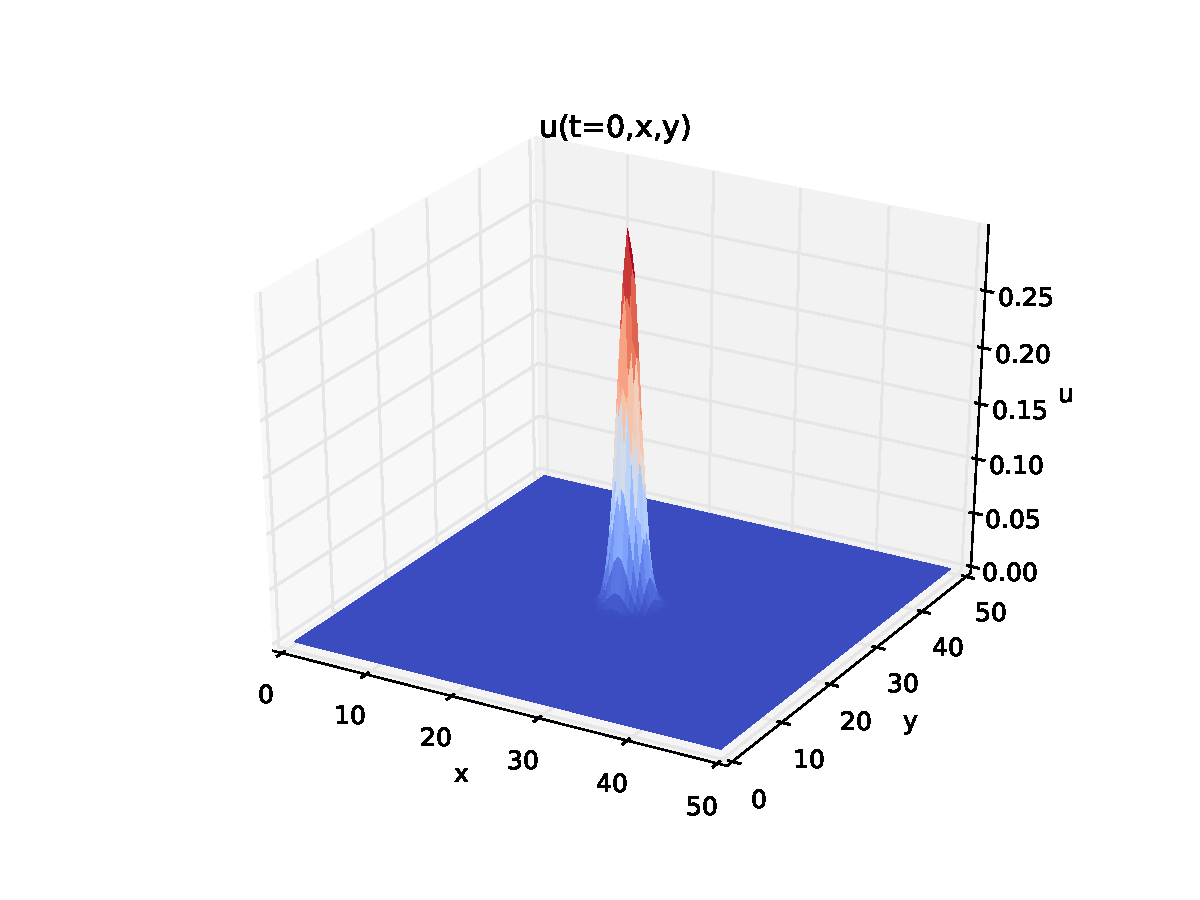
\includegraphics[width=0.5\textwidth]{Q_11_t=0.pdf}
}
\subfloat[$t = T/4$]{
  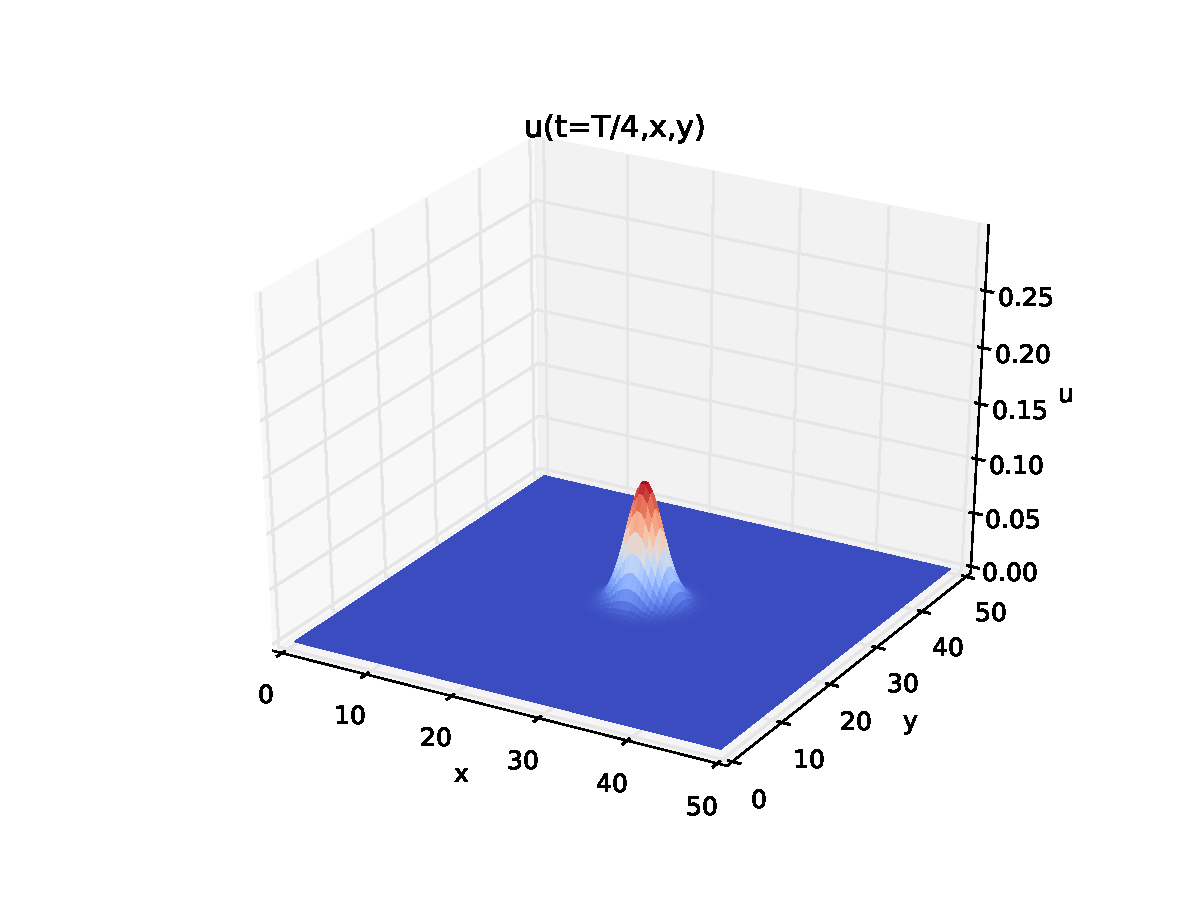
\includegraphics[width=0.5\textwidth]{Q_11_t=T-4.pdf}
}
\hspace{0mm}
\subfloat[$t = T/2$]{
  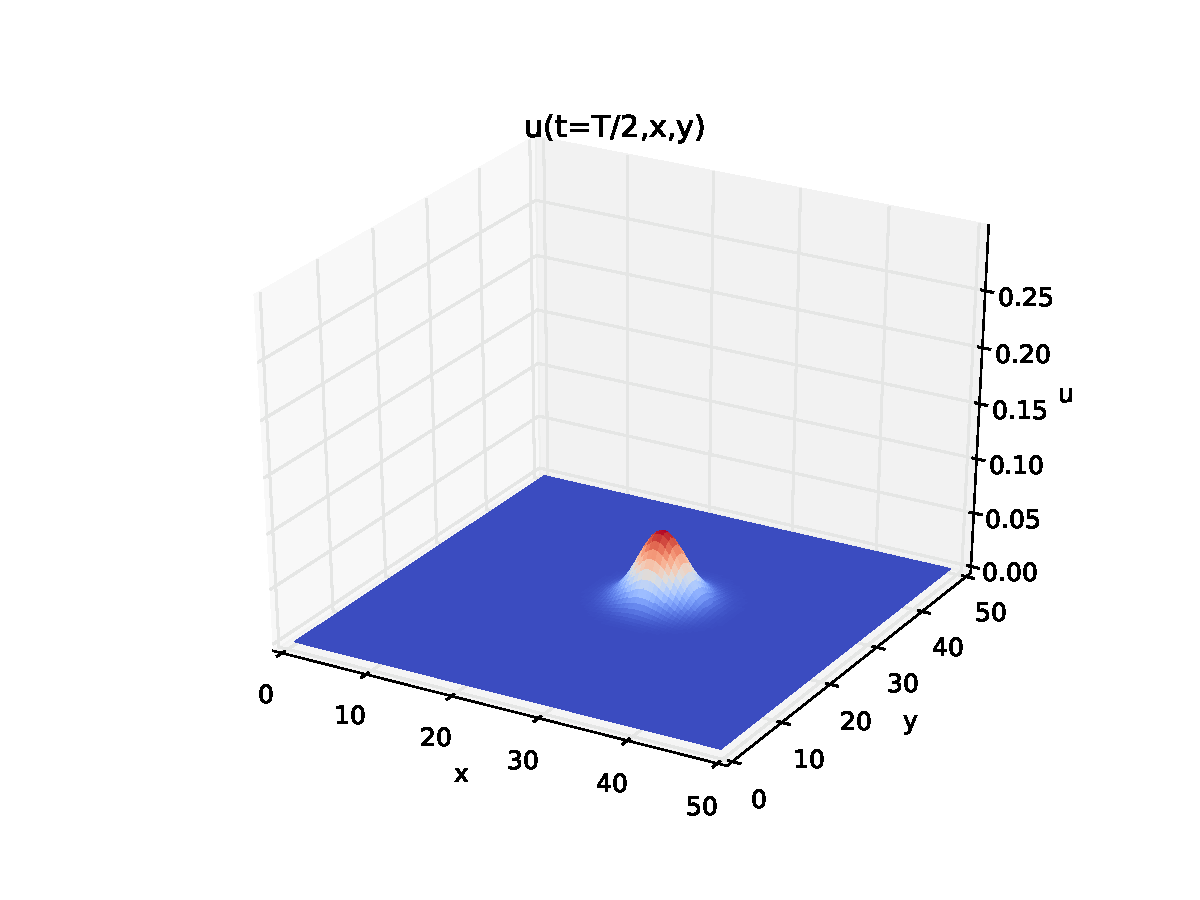
\includegraphics[width=0.5\textwidth]{Q_11_t=T-2.pdf}
}
\subfloat[$t = T$]{
  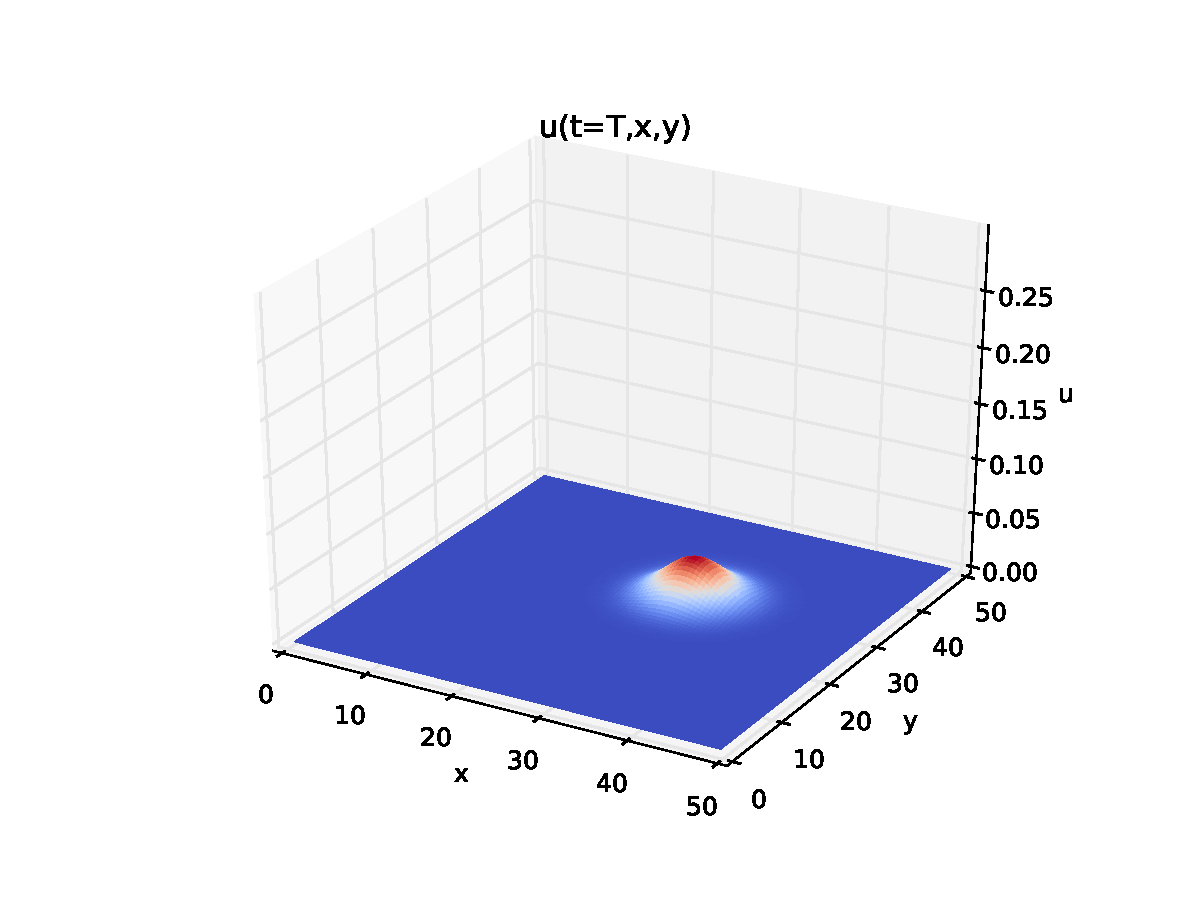
\includegraphics[width=0.5\textwidth]{Q_11_t=T.pdf}
}
\caption{Évolution en temps}
\end{figure}
\subsubsection{Q12}
Afin modéliser la dispersion du polluant dans l'océan, modifier le schéma afin de prendre en compte la participation du terme source $f = f_{x_0, y_0, \sigma}$ avec $x_0=25$ et $y_0=0$ et $\sigma = 1$.

On note le vecteur qui représente le terme de source comme $b$, un vecteur de taille $N^2$.
$$
b_{(i-1)N + j} = f(x_i, y_j) \mbox{ pour } 1 \leqslant i, j\leqslant N.
$$

Alors, l'on peut en déduire l'equation du schéma.

\begin{equation}
(I_N + \frac{\Delta t}{2}(K_c^x + K^y_c) - \frac{\nu \Delta t}{2}A)U^{n+1} = (I_N - \frac{\Delta t}{2}(K_c^x + K^y_c) + \frac{\nu \Delta t}{2}A)U^{n} + \Delta t b
\label{equ:relation_recurrence}
\end{equation}

Et l'on obtient le figure du simulation.
\newpage
\begin{figure}
\centering
\subfloat[$t = 0$]{
  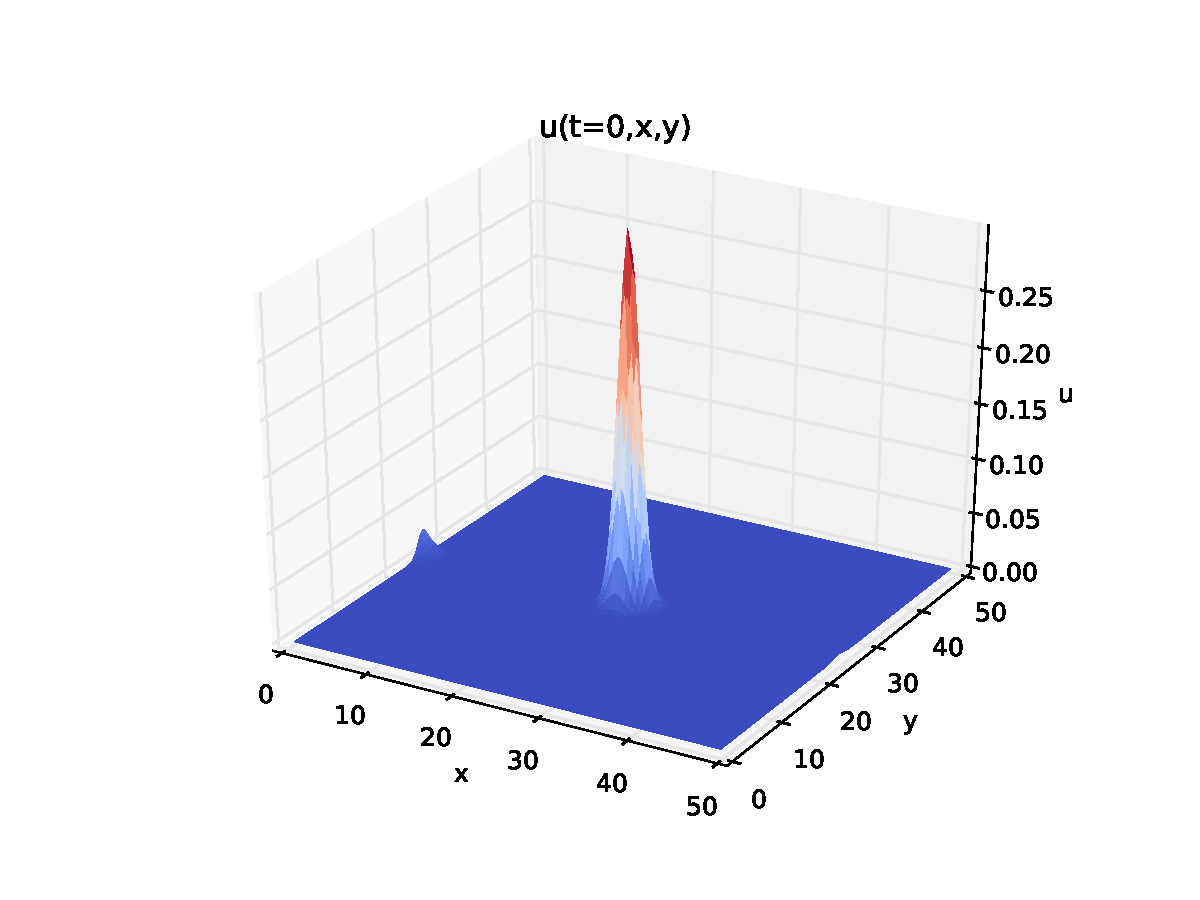
\includegraphics[width=0.5\textwidth]{Q_12_t=0.pdf}
}
\subfloat[$t = T/4$]{
  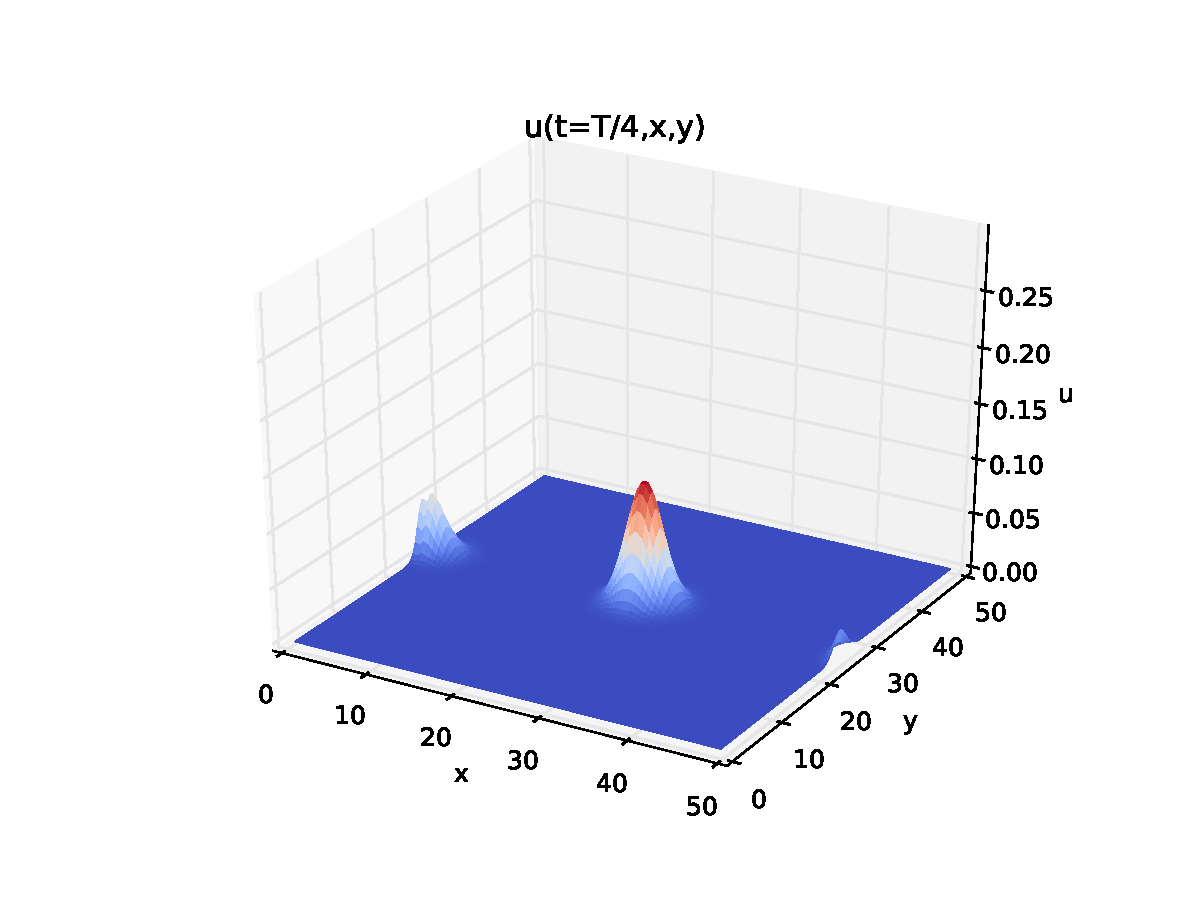
\includegraphics[width=0.5\textwidth]{Q_12_t=T-4.pdf}
}
\hspace{0mm}
\subfloat[$t = T/2$]{
  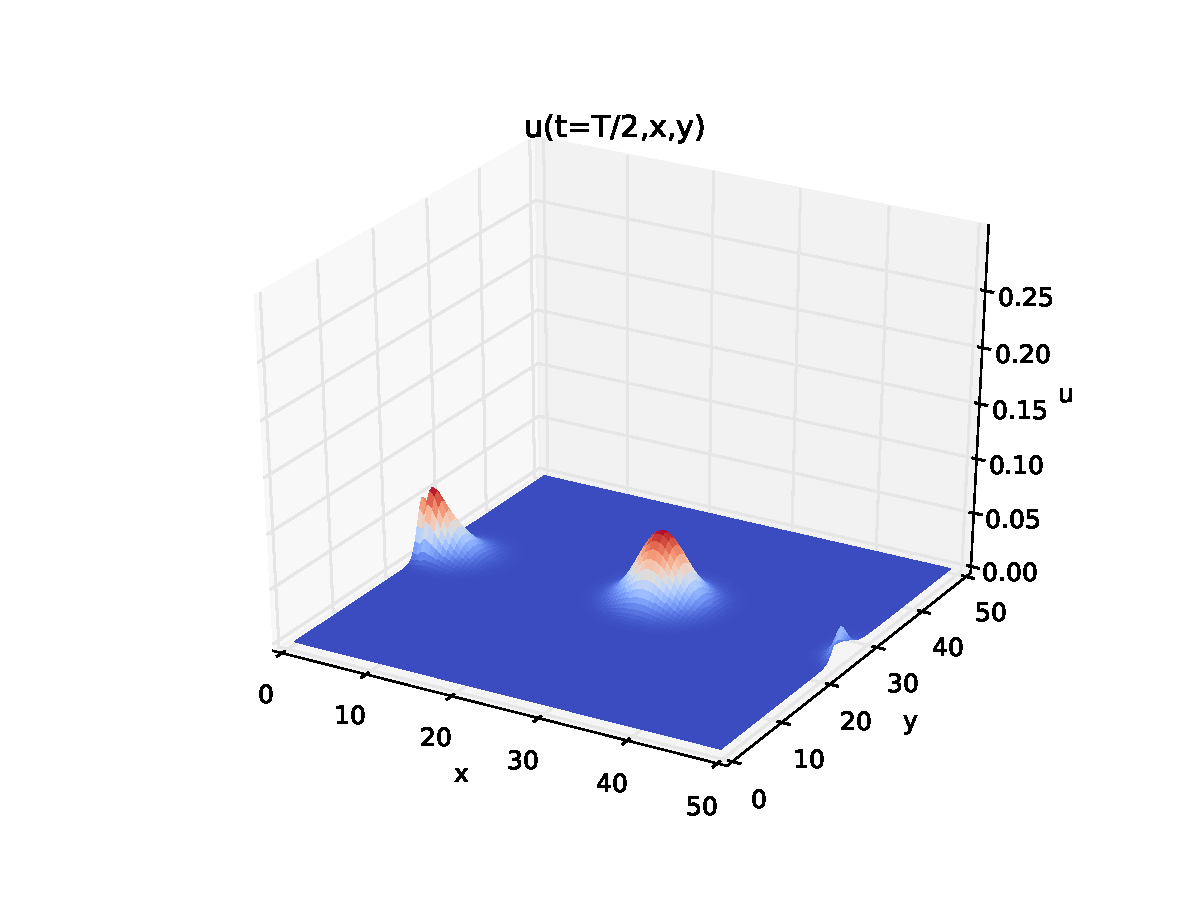
\includegraphics[width=0.5\textwidth]{Q_12_t=T-2.pdf}
}
\subfloat[$t = T$]{
  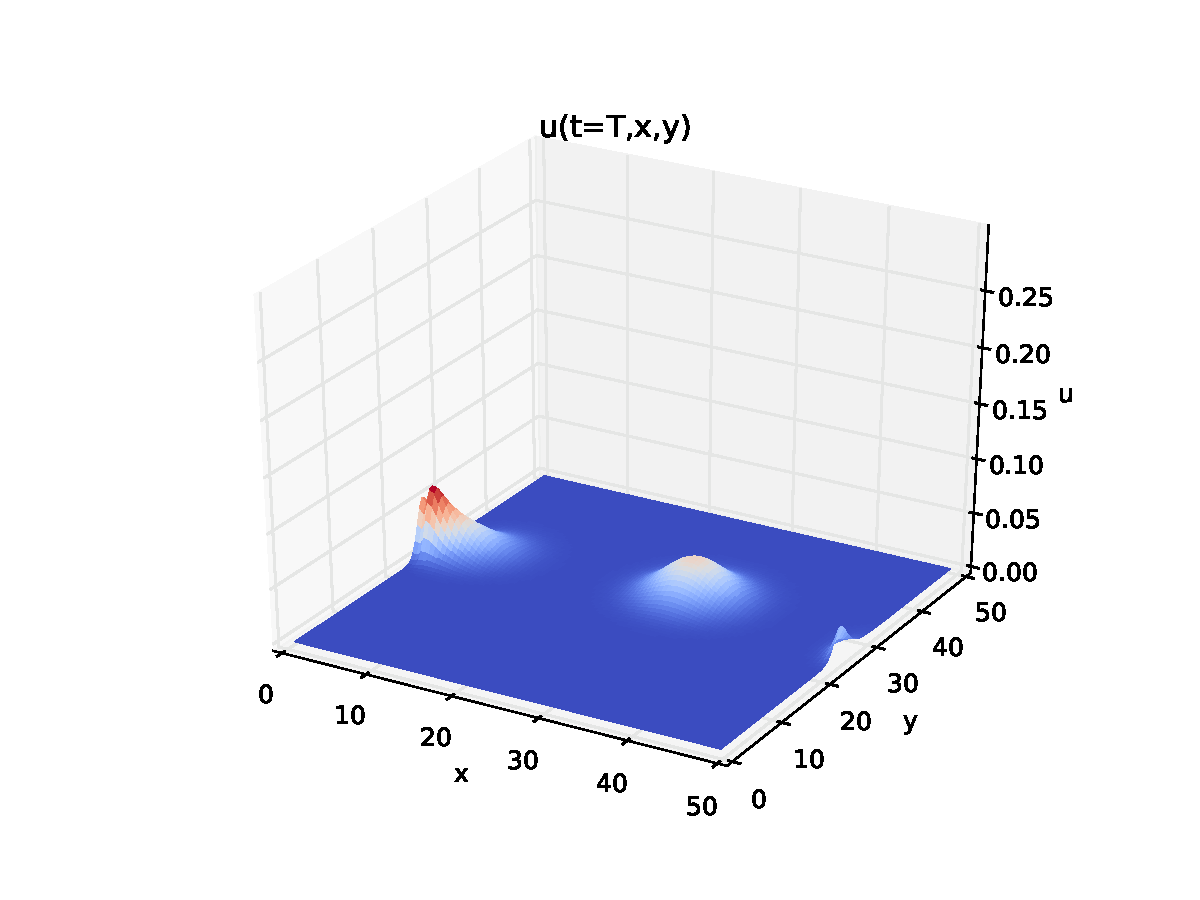
\includegraphics[width=0.5\textwidth]{Q_12_t=T.pdf}
}
\caption{Évolution en temps avec le terme de source}
\end{figure}


\subsubsection{Q13}
L'objectif final du projet est d'observer les effets du courant océaniques sur la dispersion, en particulier lorsque celui-ci dépend de la position comme à proximité de l'embouchure d'un fleuve. Modifier à présent les matrices $K_c^x$ et $K_c^y$ pour prendre en compte la dépendance de $V$ vis-à-vis de la position. Tester le nouveau schéma avec les données de la question précédente, pour le un coefficient de convection $V$ donné par

$$
V(x,y)=(\mbox{cos}(\frac{k\pi y}{L})\mbox{sin}(\frac{l\pi x}{L}),\mbox{cos}(\frac{l\pi x}{L})\mbox{sin}(\frac{k\pi y}{L})) \mbox{, avec }\forall (x,y)\in \Omega,(k,l) \in \mathbb{N}^2
$$

D'abord, on fait expliciter la forme des matrices $K_c^x$ et $K_c^y$.


\end{document}
